\subsection{Zero-Shot Performance}
\label{sec:eval:zeroshot}
Across natural language understanding and generation tasks, we find the zero-shot performance of the pretrained models to be near random chance. Figure \ref{fig:superglue} shows models' zero-shot performance, on average, across a range of prompts for a range of tasks from the SuperGLUE benchmark. Tables \ref{tab:WMT-14enfr-byprompts-0shot} and \ref{tab:mt-diabla-zero-shot-compare-baselines} show zero-shot machine translation results on English-French and English-Hindi for multiple models and datasets. We do not report zero-shot performance on summarization because generation experiments are expensive to run and, based on the results reported here and initial experiments on zero-shot summarization, it was clear the performance on summarization would be very poor. In all cases, zero-shot performance of models trained on standard language model is near chance.

\subsubsection{SuperGLUE}
On SuperGLUE, while some individual prompts show performance improvements by margins as high as 10 accuracy points, the average performance across prompts always hovers around chance, suggesting that the success of individual prompts is primarily statistical variation. The exception is the T0 model, which shows strong performance. However, this model is finetuned in the multitask setting (similar to BLOOMZ, see \Cref{sec:eval:bloomz}) in order to improve performance in zero-shot prompting settings, and thus is not directly comparable to the other models shown here.


\begin{figure}[!htbp]
    \centering
    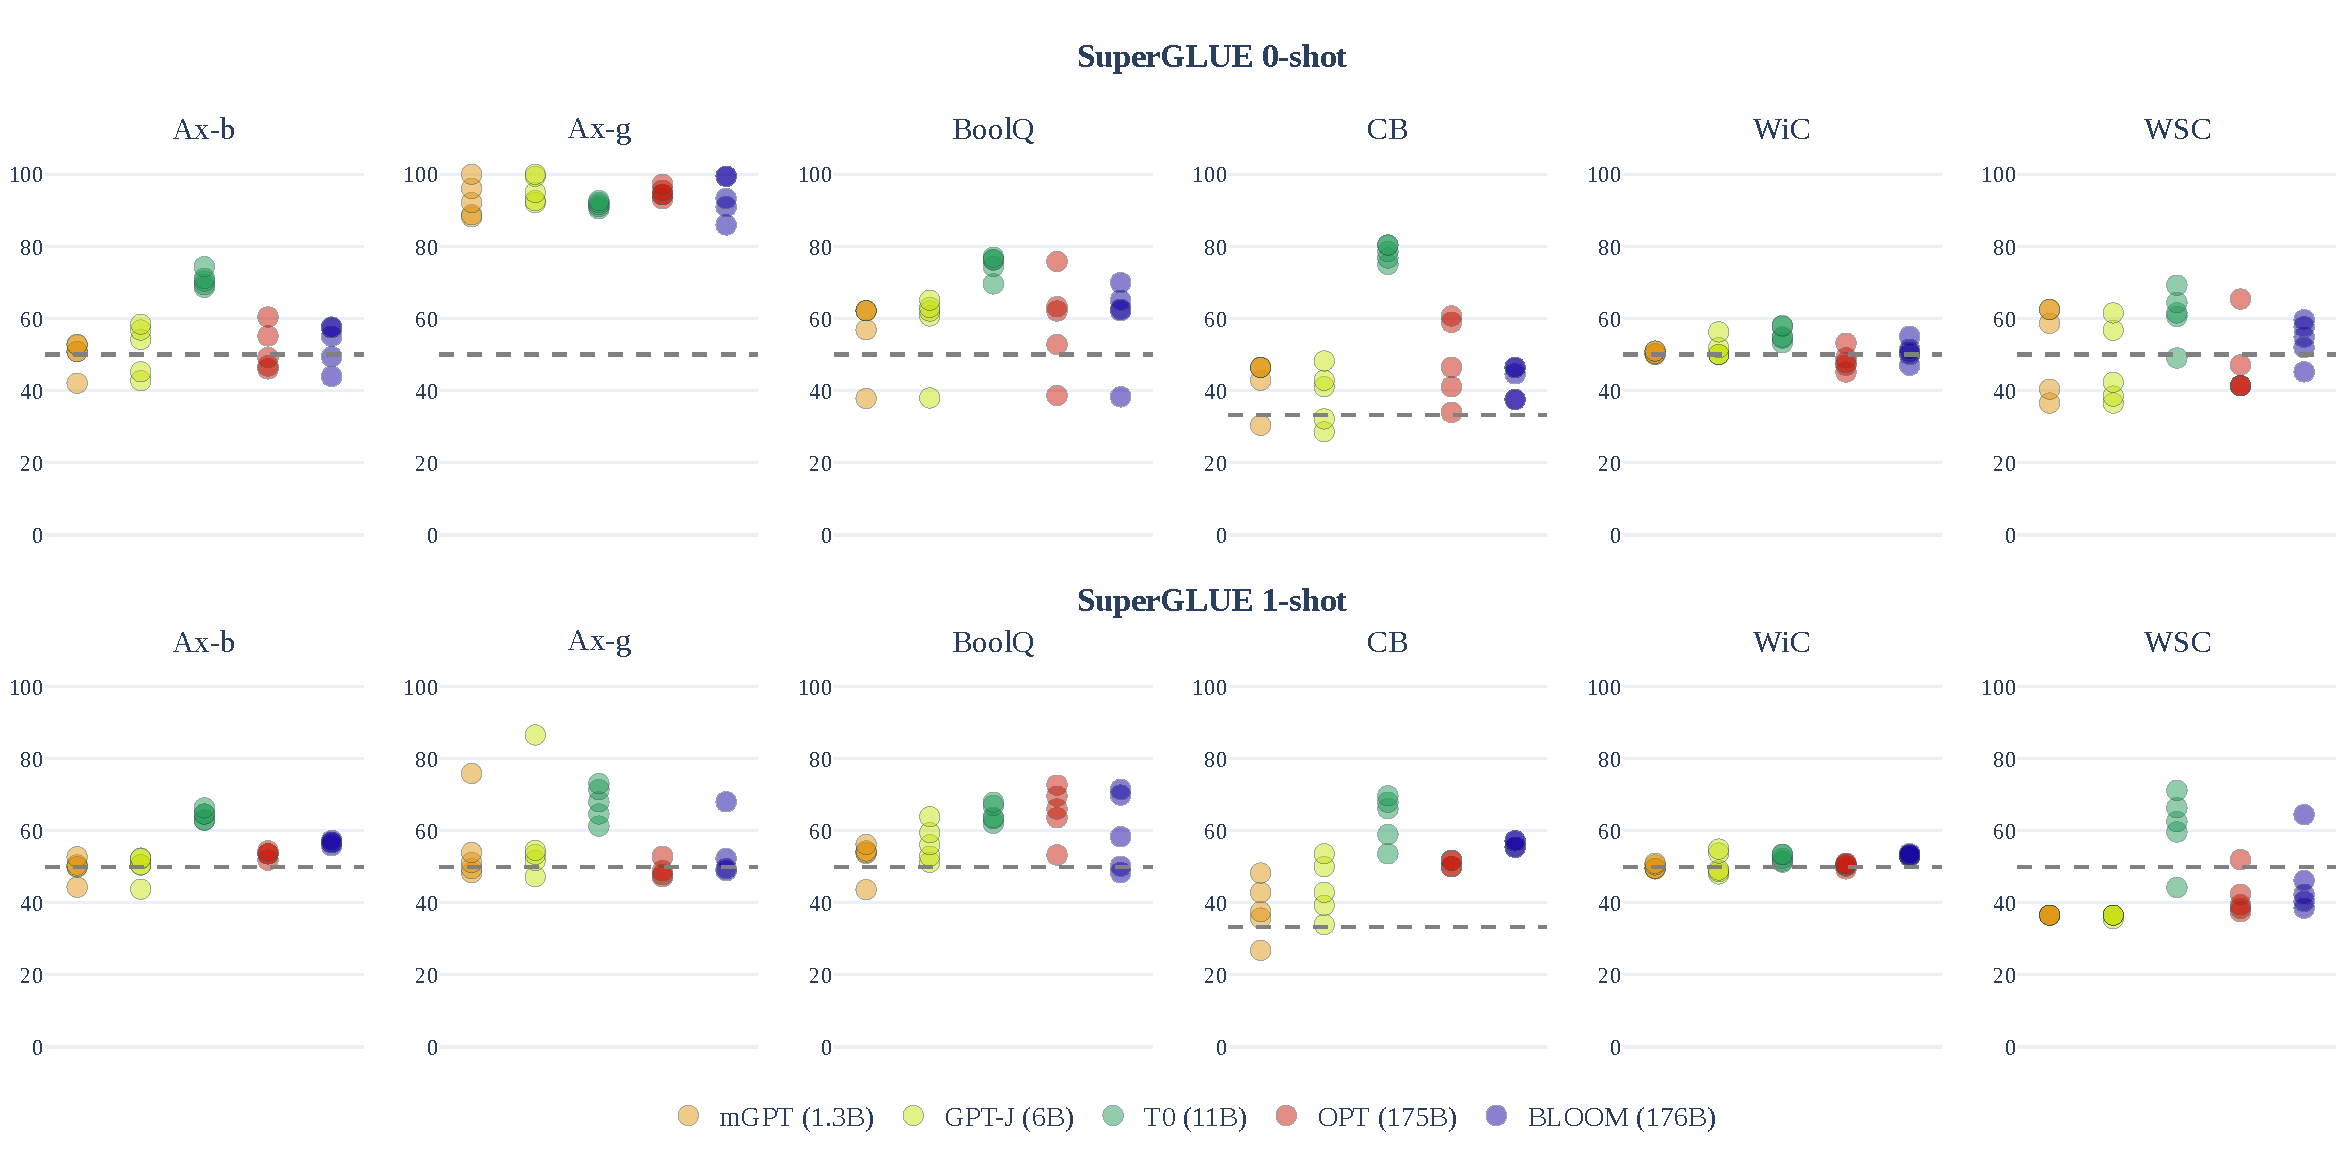
\includegraphics[width=\linewidth]{figures/super_glue.pdf}
    \caption{Performance of various LLMs on subset of tasks from SuperGLUE benchmark in zero- and one-shot prompt-based setting.}
    \label{fig:superglue}
\end{figure}




%On machine translation (MT), BLEU scores are often in the single digits, even for French-English, a high-resource language pair on which models typically are able to perform well. Both BLOOM and mGPT perform very poorly. Again T0--which is finetuned on prompts for multiple tasks (including MT)--achieves more acceptable scores (BLUE near 12), but still well below what would be necessary for the translations to be useful to humans (SOTA scores are often in the 40s). 

\subsubsection{Machine Translation}
MT results for BLOOM-176B in the zero-shot setting are given in Table~\ref{tab:WMT-14enfr-byprompts-0shot}.
%A description of the prompts can be found in Appendix~\ref{app:mt-prompt-description}.
Somewhat surprisingly the best prompts tend to be the more verbose ones. Indeed, the ``version'' prompt is consistently better and the ``gpt3'' and ``xglm'' prompts have very poor performance. 

\begin{table}[ht!]
\centering\small
\addtolength{\tabcolsep}{-2.5pt}
%\resizebox{\textwidth}{!}{
\begin{tabular}{lrr|rr|rr|rr}
\toprule
Prompt & \multicolumn{2}{c}{en $\rightarrow$ fr} & \multicolumn{2}{c}{fr $\rightarrow$ en } & \multicolumn{2}{c}{en $\rightarrow$ hi} & \multicolumn{2}{c}{hi $\rightarrow$ en} \\
% & mean & & mean &  \\
%name &  &  &      \\
\midrule
Shots  & 0 & 1 & 0 & 1 & 0 & 1 & 0 & 1 \\
\midrule
a\_good\_translation & 15.38 & 36.39 & 16.81 &  36.56 & 1.90 & 14.49 & 13.04 & 24.60  \\
gpt3     & 7.90 & 32.55 & 12.73 & 33.14 & 0.26 & 6.51 & 0.66 & 9.99 \\
version  & 21.96 & 34.22 & 26.79 & 35.42 & 1.96 & 13.95 & 11.48 & 25.81 \\
xglm     & 4.16 & 28.99 & 11.23 & 33.30 & 0.63 & 14.55 & 4.10 & 13.22 \\
\bottomrule
\end{tabular}%}
\caption{WMT'14 zero- and one-shot results for BLOOM-176B. The prompts used are described in Table~\ref{tab:prompt-examples}.}% and in more detail in Appendix~\ref{app:mt-prompt-description}.}
\label{tab:WMT-14enfr-byprompts-0shot}
\end{table}
% a\_good\_translation & 36.39 & 36.56 & 14.49 & 24.60 \\
% gpt3     & 32.55 & 33.14 & 6.51 & 9.99 \\
% version  & 34.22 & 35.42 & 13.95 & 25.81 \\
% xglm     & 28.99 & 33.30 & 14.55 & 13.22 \\

% \begin{table}[ht!]
% \centering\small
% \addtolength{\tabcolsep}{-2.5pt}
% %\resizebox{\textwidth}{!}{
% \begin{tabular}{lcccc}
% \toprule
% Prompt & en $\rightarrow$ fr & fr $\rightarrow$ en & en $\rightarrow$ hi & hi $\rightarrow$ en \\
% % & mean & & mean &  \\
% %name &  &  &      \\
% \midrule
% a\_good\_translation & 15.38  & 16.81  & 1.90  & 13.04  \\
% gpt3     & 7.90 & 12.73 & 0.26 & 0.66 \\
% version  & 21.96 & 26.79 & 1.96 & 11.48 \\
% xglm     & 4.16 & 11.23 & 0.63 & 4.10 \\
% \bottomrule
% \end{tabular}%}
% \caption{WMT'14 \textbf{zero-shot} results for BLOOM-176B. The prompts are described in Table~\ref{tab:prompt-examples}.}% and in more detail in Appendix~\ref{app:mt-prompt-description}.}
% \label{tab:WMT-14enfr-byprompts-0shot}
% \end{table}

% \begin{table}[ht!]
% \centering\small
% \addtolength{\tabcolsep}{-2.5pt}
% %\resizebox{\textwidth}{!}{
% \begin{tabular}{lcccc}
% \toprule
% Prompt & en $\rightarrow$ fr & fr $\rightarrow$ en & en $\rightarrow$ hi & hi $\rightarrow$ en \\
% % & mean & & mean &  \\
% %name &  &  &      \\
% \midrule
% a\_good\_translation & 36.39 & 36.56 & 14.49 & 24.60 \\
% gpt3     & 32.55 & 33.14 & 6.51 & 9.99 \\
% version  & 34.22 & 35.42 & 13.95 & 25.81 \\
% xglm     & 28.99 & 33.30 & 14.55 & 13.22 \\
% \bottomrule
% \end{tabular}%}
% \caption{WMT'14 \textbf{one-shot} results for BLOOM-176B. Table~\ref{tab:prompt-examples}.}% and in more detail in Appendix~\ref{app:mt-prompt-description}.}
% \label{tab:WMT-14enfr-byprompts-1shot}
% \end{table}

\begin{table}[ht!]
    \centering\small
    \begin{tabular}{lrrrcrrr}
    \toprule
    & \multicolumn{3}{c}{en $\rightarrow$ fr } & \hphantom{woo} & \multicolumn{3}{c}{fr $\rightarrow$ en } \\
    Prompt & T0 & mGPT & BLOOM && T0 & mGPT & BLOOM  \\ 
    \midrule
    MT sent-level       & 0.33 & 0.09 & 0.05 && 12.53 & 0.27 & 0.11 \\
    MT complete (1-orig-context) & 0.87 & 0.13 & 1.08 && 13.77 & 0.59 & 1.31 \\ 
    \bottomrule
    \end{tabular}
    \caption{Comparison of zero-shot results (BLEU) for DiaBLa against baseline LMs. The ``MT sent-level'' prompt requests for a translation given the source language only, whereas the ``MT complete (1-orig-context)'' prompt asks to complete a translation given the previous and current source sentences and the beginning of the translation, i.e.~the previous sentence in the target language.}
    \label{tab:mt-diabla-zero-shot-compare-baselines}
\end{table}

The two major problems observed are (i)~over-generation and (ii)~not producing the correct language (an obvious prerequisite for a good translation). These same problems can be seen with other LMs, as can be shown by the generally poor results on the DiaBla dataset shown in Table~\ref{tab:mt-diabla-zero-shot-compare-baselines}.
Despite not being a multilingual model, T0 \citep{sanh2022multitask} can sometimes perform translation into English (12.53 and 13.77 BLEU), though the fact that it is an English-based model may explain why it performs better. For BLOOM, the ``wrong-language'' problem is partially alleviated in the into-English directions by using prompts that end in the target language (as opposed to ending with the source text to translate), presumably because it is easier to generate a continuation of the prompt in the same language.
%We have so far only tested prompts in English, so this can only be validated for the into-English directions. 

\subsection{One-Shot Results}
\label{sec:eval:oneshot}

In the one-shot evaluation--where models are given a single in-context training example--we find that performance generally improves for generation tasks (MT and summarization), but not for the SuperGLUE classification tasks.

\subsubsection{SuperGLUE}
\label{sec:eval:superglue}

Figure \ref{fig:superglue} shows one-shot performance alongside the zero-shot results. As compared to zero-shot performance, one-shot performance variability to SuperGLUE is reduced across all prompts and models. Overall, there is no notable improvement associated with the one-shot setting: models average accuracy is still nearly always at chance (with the exception of T0).
%Across all 30 models, SuperGLUE task combinations, only about a third (n=11) increase in average accuracy, but the differences are.
%A notable exception to this trend WSC; none of the models tested increase in average accuracy across prompts. An exception to this trend is BLOOM, which increases from zero-shot to one-shot for every SuperGLUE task, except WSC.  None of the models tested had an increase in performance when evaluated on WSC. 

We perform an additional analysis comparing BLOOM models across model sizes.  As a baseline, we also measure the average one-shot accuracy of OPT models of similar sizes (350M parameters to 175B parameters).\footnote{We do not evaluate OPT-66B because of the lack of a similarly-sized BLOOM model.} Figure \ref{fig:superglue-scaling} shows the accuracy of each prompt on each task across model scales. Both OPT and BLOOM model families improve slightly with scale, and there is no consistent difference between families across all tasks. BLOOM-176B is ahead of OPT-175B on Ax-b, CB and WiC. %The performance of BLOOM is comparable to OPT across SuperGLUE tasks, suggesting that multilinguality does not limit performance of BLOOM on English-only tasks.

\begin{figure}[ht!]
    \centering
    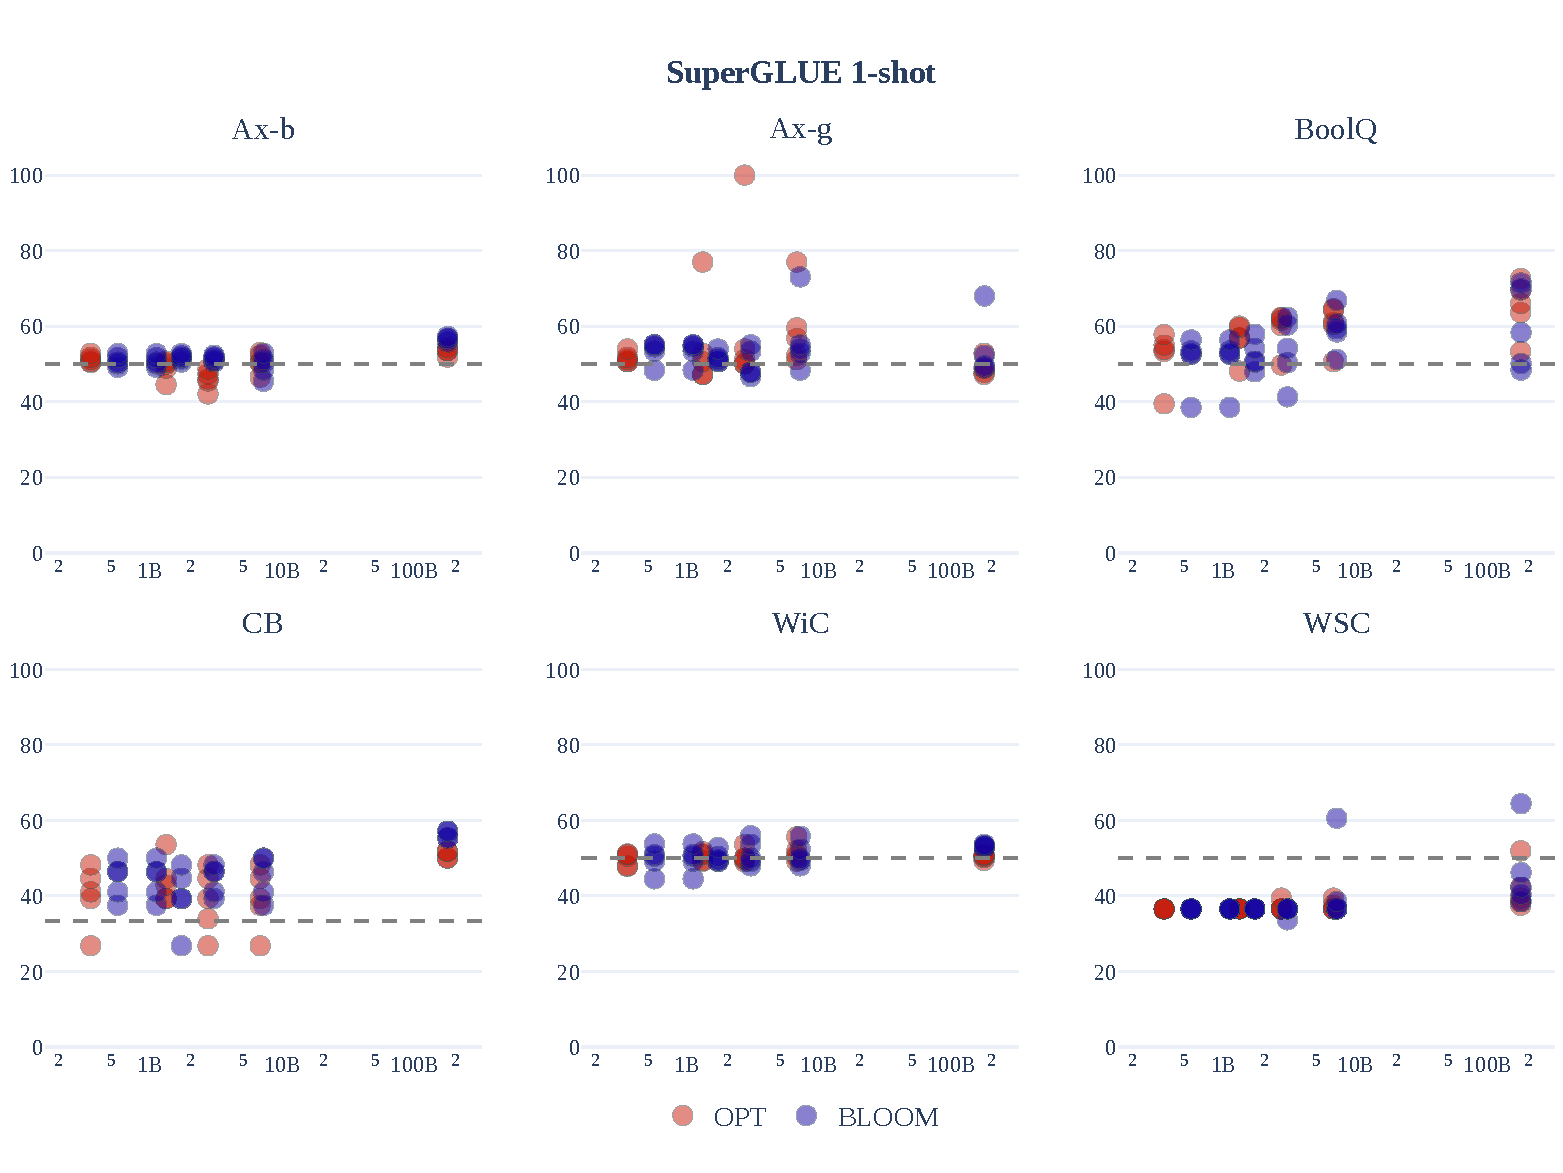
\includegraphics[width=\linewidth]{figures/super_glue_params.pdf}
    \caption{Comparison of the scaling of BLOOM versus OPT on each SuperGLUE one-shot task. Each point represents the average accuracy of a model within the BLOOM or OPT family of models on one of the five task prompts. The number of parameters on the x-axis is presented in log-scale.}
    \label{fig:superglue-scaling}
\end{figure}

\subsubsection{Machine Translation}
\label{sec:eval:mt}

In the 1-shot setting, we test several language directions in the Flores-101 \citep{goyal-etal-2022-flores} devtest set using the XGLM prompt \citep{lin2021xglm}.%, provided in Appendix~\ref{app:mt-prompt-description}).
We choose the 1-shot example randomly from the same dataset, which may differ from past work.
We separate out results for high-resource language pairs (\Cref{tab:flores101_summary:high-high}), high-to-mid-resource language pairs (\Cref{tab:flores101:high-mid}), low-resource language pairs (\Cref{tab:flores101_summary:high-low}) and between related languages of the Romance language family (\Cref{tab:flores101_summary:same-fami}).%--more complete results for more languages are given in Appendix~\ref{app:mt-one-shot}.
 Languages are classified as low-, mid- and high-resource depending on their representation in ROOTS.
%Results for high-resource language pairs and for pairs involving translation from a high- to a mid-resource language are shown in Table~\ref{tab:flores101_summary:high-high} and Table~\ref{tab:flores_summary-high-midhigh-results} respectively. 
For high- and mid-to-high-resource pairs, we compare to supervised results from the M2M-124 model \citep{fan-etal-2021-beyond} with 615M parameters, for which scores are computed by \cite{goyal-etal-2022-flores}. Additionally, we compare to XGLM (7.5B) 1-shot results \citep{lin2021xglm} and 32-shot AlexaTM results \citep{soltan-etal-2022-alexatm}. %As above, all scores for Flores-101 are calculated using spBLEU as recommended for this dataset, using \texttt{sacrebleu} and spm-flores-101 tokenisation.
%
Results are good across the board for both translation between high-resource languages and from high- to mid-resource languages, suggesting BLOOM's good multilingual capacity, even across scripts (here between Latin (or extended Latin), Chinese, Arabic and Devanagari scripts). Comparing against the supervised M2M model, results are often comparable and sometimes better in this 1-shot setting, and results are comparable in many cases to those of AlexaTM.

The translation quality for many of the low-resource languages is good, comparable or even slightly better than the supervised M2M model.
%\footnote{Results are for the M2M-124 615M model~\citep{fan-etal-2021-beyond} as computed by \cite{goyal-etal-2022-flores}.} 
However, results are very poor between Swahili and Yoruba, languages that are present but under-represented in BLOOM's training data ($<$50k tokens each). This contrasts with the results for translation between Romance (and therefore related) languages, where results are good across-the-board, including for translation from Galician (glg), a language not included in the training data, but which shares many similarities with the other Romance languages, in particular with Portuguese (por). This however does question BLOOM's quality on those under-represented low-resource languages included in training.

\begin{table}[!ht]
 \centering\footnotesize
 \begin{subtable}[t]{0.48\textwidth}
 \scalebox{0.86}{
  \begin{tabular}{llrrrrr}
  \toprule
  Src$\downarrow$ & Trg$\rightarrow$ & eng & ben & hin & swh & yor  \\
  \midrule
  \multirow{2}{*}{eng}
  & M2M & -- & 23.04 & 28.15 & 29.65 & 2.17  \\
  %& mT0 & \\
  & BLOOM & -- & 25.52 & 27.57 & 21.7 & 2.8 \\
  \midrule
  \multirow{2}{*}{ben}
  & M2M & 22.86 & -- & 21.76 & 14.88 & 0.54  \\
  %& mT0 & \\
  & BLOOM & 30.23 & -- & 16.4 & -- & -- \\
  \midrule
  \multirow{2}{*}{hin}
  & M2M & 27.89 & 21.77 & -- & 16.8 & 0.61  \\
  %& mT0 & \\
  & BLOOM & 35.40 & 23.0 & -- &-- & -- \\
  \midrule
  \multirow{2}{*}{swh}
  & M2M & 30.43 & 16.43 & 19.19 & -- & 1.29 \\
  %& mT0 & \\
  & BLOOOM & 37.9 & -- & -- & -- & 1.43 \\
  \midrule
  \multirow{2}{*}{yor}
  & M2M & 4.18 & 1.27 & 1.94 & 1.93 & -- \\
  %& mT0 & \\
  & BLOOM & 3.8 & -- & -- & 0.84 & -- \\
  \bottomrule
\end{tabular}}
\caption{Low-resource languages}
\label{tab:flores101_summary:high-low}
\end{subtable}
%
\hfill
%
 \begin{subtable}[t]{0.48\textwidth}
 \centering\footnotesize
  \scalebox{0.86}{
 \begin{tabular}{llrrrr}
    \toprule
    Src$\downarrow$ & Trg$\rightarrow$  & cat & spa & fre & por  \\
    \midrule
    \multirow{2}{*}{cat}
    & M2M & -- & 25.17 & 35.08 & 35.15  \\
    % & GPT-3 6.7B & 32 & & & & & & & & & & & & \\
    %& mT0 \\
    & BLOOM & -- & 29.12 & 34.89 & 36.11  \\
    \midrule
    \multirow{2}{*}{spa}
    & M2M & 23.12 & -- & 29.33 & 28.1 \\
    % & GPT-3 6.7B & 32 & & & & & & & & & & & & \\
    %& mT0 \\
    & BLOOM & 31.82 & -- & 24.48 & 28.0  \\
    \midrule
    \multirow{2}{*}{glg}
    & M2M & 30.07 & 27.65 & 37.06 & 34.81 \\
    % & GPT-3 6.7B & 32 & & & & & & & & & & & & \\
    %& mT0 \\
    & BLOOM & 38.21 & 27.24 & 36.21 & 34.59  \\
    \midrule
    \multirow{2}{*}{fre}
    & M2M & 28.74 & 25.6 & -- & 37.84 \\
    % & GPT-3 6.7B & 32 & & & & & & & & & & & & \\
    %& mT0 \\
    & BLOOM & 38.13 & 27.40 & -- & 39.60 \\
    \midrule
    \multirow{2}{*}{por}
    & M2M & 30.68 & 25.88 & 40.17 & --  \\
    % & GPT-3 6.7B & 32 & & & & & & & & & & & & \\
    %& mT0 \\
    & BLOOM &  40.02 & 28.1 & 40.55 & -- \\
    \bottomrule
  \end{tabular}}
\caption{Romance languages}
\label{tab:flores101_summary:same-fami}
\end{subtable}

\vspace{1em}

\begin{subtable}[b]{0.48\textwidth}
 \centering\footnotesize
\scalebox{0.85}{
\begin{tabular}{llrrrrr}
\toprule
 Src $\downarrow$ & Trg $\rightarrow$ & ara & fre & eng & chi & spa \\
\midrule
\multirow{4}{*}{ara}
  & M2M & -- & 25.7 & 25.5 & 13.1 & 16.74  \\
  %& GPT-3 6.7B & 32 & & & & & & & & & & & & \\
  & XGLM & -- & 17.9 & 27.7 & --  & --  \\
  & AlexaTM & -- & 35.5 & 41.8 & -- & 23.2 \\
  & BLOOM & -- & 33.26 & 40.59 & 18.88 & 23.33\\
\midrule
\multirow{4}{*}{fre}
  & M2M & 15.4 & -- & 37.2 & 17.61 & 25.6  \\
  %& GPT-3 6.7B & 32 & & & & & & & & & & & & \\
  & XGLM & 5.9 & -- & 40.4 & -- &  --\\
  & AlexaTM & 24.7 & -- & 47.1 & -- & 26.3   \\
  & BLOOM & 23.30 & -- & 45.11 & 22.8 & 27.4 \\
\midrule
\multirow{4}{*}{eng}
  & M2M & 17.9 & 42.0 & -- & 19.33 & 25.6  \\
  %& GPT-3 6.7B & 32 & & & & & & & & & & & & \\
  & XGLM & 11.5 & 36.0 & -- & -- & --  \\
  & AlexaTM & 32.0 & 50.7 & -- & -- & 31.0  \\
  & BLOOM & 28.54 & 44.4 & -- & 27.29  & 30.1 \\
\midrule
\multirow{4}{*}{chi}
  & M2M & 11.55 & 24.32 & 20.91 & -- & 15.92 \\
  %& GPT-3 6.7B & 32 & & & & & & & & & & & & \\
  & XGLM & -- & -- & -- & -- & -- \\
  & AlexaTM & -- & -- & -- & -- & -- \\
  & BLOOM & 15.58 & 25.9 & 30.60 & -- &  20.78 \\
\midrule
\multirow{4}{*}{spa}
  & M2M & 12.1 & 29.3 & 25.1 & 14.86 & --  \\
  %& GPT-3 6.7B & 32 & & & & & & & & & & & & \\
  & XGLM & -- & -- & -- & -- & -- \\
  & AlexaTM & 20.8 & 33.4 & 34.6 & ?? & --  \\
  & BLOOM & 18.69 & 24.48 & 33.63 &  20.06 & -- \\
\bottomrule
\end{tabular}}
\caption{High-resource language pairs.}
\label{tab:flores101_summary:high-high}
\end{subtable}
%
\hfill
%
\begin{subtable}[b]{0.48\textwidth}
\centering\footnotesize
\scalebox{0.85}{
\begin{tabular}{llrrrrr}
  \toprule
  Src $\downarrow$ & Trg $\rightarrow$ & eng & fre & hin & ind & vie  \\
  \midrule
  \multirow{2}{*}{eng}
  & M2M & -- & 41.99 & 28.15 & 37.26 & 35.1  \\
  % & GPT-3 6.7B & 32 & & & & & & & & & & & & \\
  %& mT0 \\
  & BLOOM & -- & 44.4 & 27.57 & 38.75 &28.83\\
  \midrule
  \multirow{2}{*}{fre}
  & M2M & 37.17 & -- & 22.91 & 29.14 & 30.26  \\
  % & GPT-3 6.7B & 32 & & & & & & & & & & & & \\
  %& mT0 \\
  & BLOOM & 45.11 & -- & 17.04 & 29.50  & 31.66 \\
  \midrule
  \multirow{2}{*}{hin}
  & M2M  & 27.89 & 25.88 & -- & 21.03 & 23.85  \\
  % & GPT-3 6.7B & 32 & & & & & & & & & & & & \\
  %& mT0 \\
  & BLOOM & 35.40 & 27.83 & -- &  --  & -- \\
  \midrule
  \multirow{2}{*}{ind}
  & M2M & 33.74 & 30.81 &  22.18 & -- & 31.4 \\
  % & GPT-3 6.7B & 32 & & & & & & & & & & & & \\
  %& mT0 \\
  & BLOOM & 44.59 & 29.75 & -- & --  & -- \\
  \midrule
  \multirow{2}{*}{vie}
  & M2M & 29.51 & 28.52 & 20.35 & 27.1 & --  \\
  % & GPT-3 6.7B & 32 & & & & & & & & & & & & \\
  %& mT0 \\
  & BLOOM & 38.77 & 28.57 & -- & --  & -- \\
  \bottomrule
\end{tabular}}
\caption{High$\rightarrow$mid-resource language pairs.}
\label{tab:flores101:high-mid}
\end{subtable}
\caption{\label{tab:flores-results}1-shot MT results (spBLEU) on the Flores-101 devtest set. }
\end{table}

\subsubsection{Summarization}
\label{sec:eval:wikilingua}

%Results.
Figure \ref{fig:wikilingua} shows one-shot results for BLOOM models alongside OPT-175B for comparison. Each point represents a per-prompt score. The key takeaways are that BLOOM attains higher performance on multilingual summarization than OPT and that performance increases as the parameter count of the model increases. We suspect this is due to BLOOM's multilingual-focused training.

\begin{figure*}[ht!]
    \centering
    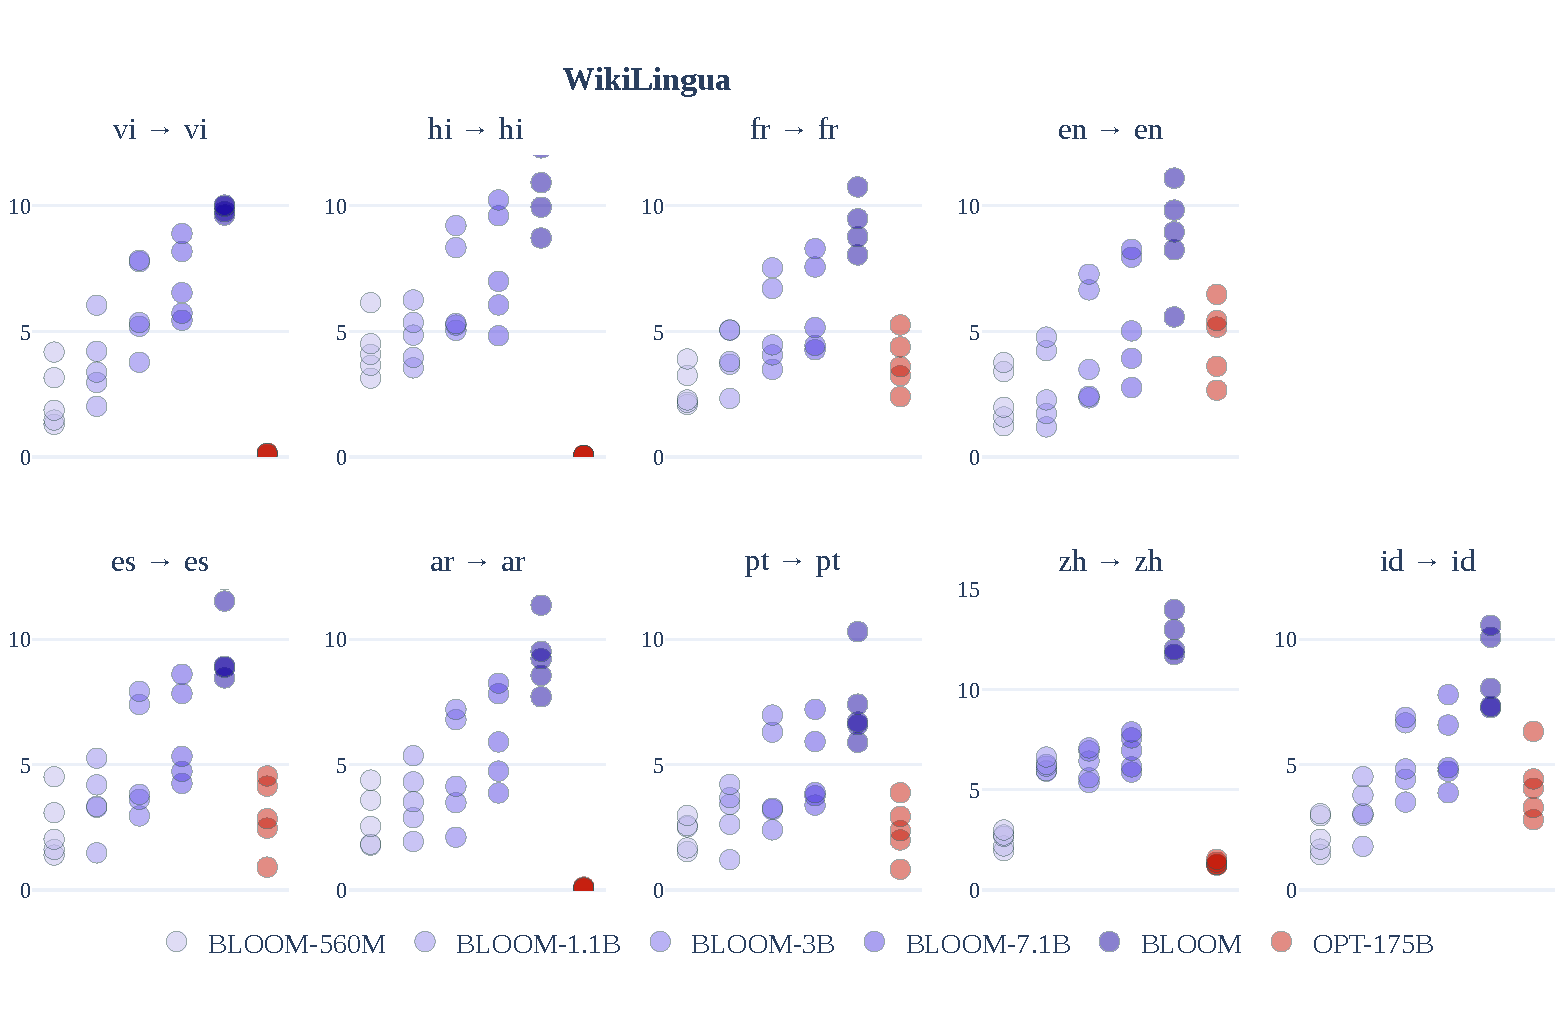
\includegraphics[width=\linewidth]{figures/wikilingua_fewshot_results_zh_id.pdf}
    \caption{WikiLingua One-shot Results. Each plot represents a different language with per-prompt ROUGE-2 F-measure scores.}
    \label{fig:wikilingua}
\end{figure*}

As discussed in Section \ref{sec:eval:design}, we report ROUGE-2 scores for the sake of comparability with prior work, and because there is a lack of alternatives for generation evaluation. 
%We also report ROUGE-L and Levenshtein distance in Tables \ref{tab:wikilingua_rougeL_table}, \ref{tab:wikilingua_lev_dist_table}.
However, we qualitatively observe that in many cases, the ROUGE-2 score understates the quality of the summaries generated by the systems.